;\chapter{Network Error Logging a relevantné technológie}
\label{nel-and-related-technologies}

% TODO:
% \begin{enumerate}
%     \item Prezriet GFG ohladom internetu
%     \item Zavolať s Petrom ohľadom predstavy, ako chcem napísať úvod o "Internete"
%     \item Postupne spísať po Report API
%     \item Naštudovať podklady k Report API LEPŠIE, aby som presne vedel čo chcem spomenúť
%     \item Revisit kapitoly 3
%     \item Spisat 4
%     \item Review a uhladit si pohlad na vec, aby som spravil navrh
%     \item Spisat draft navrhu
%     \item Dotiahnut data
%     \item Upravit navrh
% \end{enumerate}


% ....Uvod do kapitoly 1....

% POZNAMKY:

% the global system of interconnected computer networks
% Internet, a system architecture that has revolutionized mass communication, mass media, 
% and commerce by allowing various computer networks around the world to interconnect. Sometimes referred to as a “network of networks,”

% the world wide web is an information retrieval service of the web. It provides users with a huge array of documents that are connected to each other 
% by means of hypertext or hypermedia links. Here, hyperlinks are known as electronic connections that link the related data so that users can easily access 
% the related information hypertext allows the user to pick a word or phrase from text, and using this keyword or word or phrase can access 
% other documents that contain additional information related to that word or keyword or phrase. World wide web is a project which is created by Timothy Berner’s 
% Lee in 1989, for researchers to work together effectively at CERN. It is an organization, named World Wide Web Consortium (W3C), 
% which was developed for further development in the web.


% %##########################################################

% Príbeh kapitoly 2.:

% \# Prostredie
% Web (WWW)                           OK
% Web klient        
% Web server                          OK

% \# Identifikácia Komunikanta
% Doména
%     Sub-Doména
%     TLD
%     eTLD
%     Verejný Suffix
% IP Adresa
% DNS
%     DNS Server
%     Rezolúcia
% URL                                 OK
%     https://url.spec.whatwg.org/


% \# Komunikácia
% HTTP, HTTPS
% User Agnet
% Hlavičky
% Request
% Response

% \# Existujúce komunikačné riešenia
% Webová služba ???
% Webová stránka
%     Webová podstránka
%     Priamy Odkaz                    OK
%     Spätný Odkaz ???
%     Resource - zdroje stránky
% Dosiahnuteľnosť Web Serveru

% \# Sprostredkovanie komunikácie
% Prehliadač
%     JavaScript
%     Web API

% \# Meraná veličina v analýze
% Stav Webu
%     SEO

% \# Toto asi netreba
% Bezpečnosť na WEBe
%     Google Safe Browsing ???

% \# Aký problém vzniká
% Zlyhanie komunikácie
%     Bežné, detekovateľné (HTTP 400, 500)
%     Nedetekovateľné (Elaborate pls)

% \# Riešenie číslo 1. Nedostatočné
% Reporting API
%     Riešenie pre čo 
%     Ako
%     Nedostatky

% \# Riešenie na mieru - Subjekt analýzy    
% NEL


% %##########################################################


% Ešte raz, ale iba koncepty bez nutnej postupnosti v texte: 
% www ako sluzba
%     Domeny
%         Typy Domen
%         Kde su spisane
%         DNS
%         URL
    
% HTTP
%     Klient Server
%     Request
%     Response
%     Headers
%     Content
%         HTML
%         HyperLink / HyperText
%         Web Resource
%         MediaType
%     Browser
%         JS
    
% Problemy v Komunikacii so serverom
%     ?
%     Report Api
%         Popis
%         Nedostatky

% Network Error Logging
%     Popis


Network Error Logging (ďalej už iba \textbf{NEL}) je technológia využívaná vo web prostredí, 
kde má svoju rolu v monitorovaní špecifických problémov komunikácie zariadení pripojených do webu.
Pre plné pochopenie čím je technológia NEL v tejto kapitole vysvetľujem najprv 
spomínané prostredie, v ktorom figuruje. 
V prvom rade sa teda zameriavam na terminológiu, ktorá sa v nadchádzajúcich častiach tejto práce fekventovane používa. 

Následne sa dostanem k definícii problémov, ktoré bežne vznikajú pri komunikácií
zariadení na webe.
Pri nich spomeniem, aké riešenia predchádzali technológiu NEL a kde zlyhávali.

Samotný popis pre NEL nasleduje za úvodom do jeho závislosti, \textbf{Reporting API}, bez ktorej samostatne nemôže fungovať.

\section{Webové prostredie}

V rámci internetu, globálnej infraštruktúry sieťou prepojených zariadení, ktorá tvorí takzvanú sieť sietí, existuje systém World Wide Web (ďalej už iba web).
Web je služba ponúkajúca možnosť získavať dokumenty uložené na internete, a teda na zariadeniach do neho pripojených, nazývaných taktiež \textbf{web server}. 
Vyhľadávanie a získavanie spomínaných dokumentov, a teda obsahu dostupného na web serveri, funguje na základe ich vzájomného prepojenia takzvanými hyperlinkami.
Termín \textbf{hyperlink} v tomto kontexte prestavuje taký odkaz na dokument, ktorý umožňuje tento dokument identifikovať, lokalizovať a získať z webu. 
Hyperlinky sa vyskytujú ako súčasti obsahu získavaného dokumentu, a to vo forme či už textu (\textbf{hypertext}) alebo rôznych iných typov médií (\textbf{hypermédiá}), ako napríklad obrázky, videá alebo reklamy. 


\begin{figure}[htb]
\begin{center}
 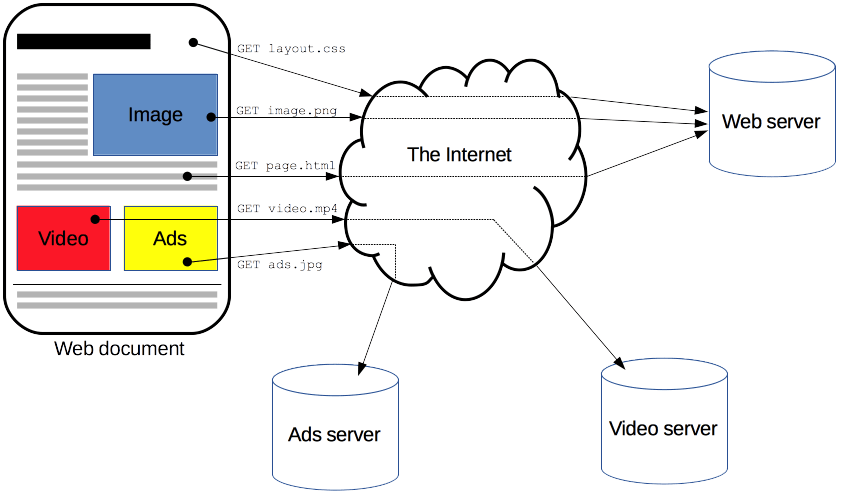
\includegraphics[scale=0.49]{obrazky-figures/fetching_a_page.png}
 \caption{\centering Vizualizácia webového prostredia. Za využitia infraštruktúry internetu prepája pomocou hyperlinkov dokumenty, ktoré možno na webe prehliadať.}
 \label{img:fetching-a-page}
\end{center}
\end{figure}

\todo{cite the images}

\pagebreak

\subsection{Navigácia na webe}

Hyperlinky na iné dokumenty sú formované ako reťazcová hodnota nazývaná Uniform Resource Locator (jednotný lokátor zdrojov, ďalej už iba \textbf{URL}).
Vďaka hodnotám URL je možné odkazovať sa na obsah webu, prepájať rôzne dokumenty medzi sebou, a tým pádom web navigovať.
Typická hodnota URL sa skladá zo:
\begin{enumerate}
    \item schémy - označenie protokolu používaného na sieťovú komunikáciu medzi servermi,
    \item domény
    \item a cesty k uloženému dokumentu.
\end{enumerate}

\begin{figure}[htb]
\begin{center}
 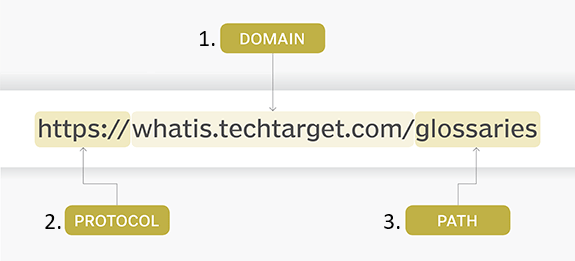
\includegraphics[scale=0.6]{obrazky-figures/the-anatomy-of-a-url.png}\label{fig:figure1}
 \caption{\centering Základná štruktúra hodnoty URL. Hodnoty bývajú rôzne a skladajú sa taktiež z niekoľkých ďalších častí, no tie však nie je potrebné pre účely tejto práce rozoberať.}
 \label{img:urlstructure}
\end{center}
\end{figure}

\pagebreak

Tieto hlavné zložky hodnôt URL predstavujú samostatne dôležité koncepty pre navigáciu vo webe.
Protokol (1.) definuje možinu platných pravidiel pre komunikáciu zariadenia návštevníka webu s web 
serverom, ktorého prislúchajúce meno je definované ďalšou časťou URL --- doménou (2.). 
Cestu k uloženému dokumentu (3.) web server interpretuje podľa jeho konfigurácie ako navigačné inštrukcie 
v rámci jeho vlastného, alebo vzdialeného úložiska jemu sprístupneného. 
Podľa týchto inštrukcií vyberie server vyžiadaný dokument a zašle ho naspäť spomínanému návštevníkovi webu.
V ďalších kapitolách do tohto procesu nahliadam hlbšie.


\subsection{Protokol HTTP(S)}
Definíciou, v oblasti sietí termín protokol predstavuje štandardizovanú množinu pravidiel pre vzájomnú komunikáciu medzi počítačovými zariadeniami. % \ref{}
Vzhľadom na to, že funkčnosť technológie NEL sa zakladá na komunikácií za pomoci protokolu HTTPS, % \ref{}
venujem sa v tejto sekcií výhradne protokolom HTTP a jeho zabezpečenej, uvedenej verzii --- HTTPS. 

% \ref{https://www.rfc-editor.org/rfc/rfc9110.html}
HTTP, celým názvom HyperText Transfer Protokol, je bezstavový aplikačný protokol pre distribuované hypertextové informačné systémy. 
Poskytuje jednotné komunikačné rozhranie pre prenos dokumentov (daľej v terminológií špecifikácie HTTP už iba ako \textbf{zdroj}).
Toto rozhranie definuje dva typy zasielateľných správ --- \textbf{žiadosť} a \textbf{odpoveď}. Žiadosť predtavuje doslova žiadosť o zdroj. Odpoveď je reakciou na žiadosť, kde je možné, že sa navráti buď žiadaný zdroj, alebo popis chyby, ktorá vznikla pri pokuse o jeho navrátenie. 

Protokol funguje na základe klient-server komunikácie, kde klient a server sú názvy rolí, ktoré môžu prepojené zariadenia zaujať v rámci komunikácie pomocou HTTP:
\begin{itemize}
    \item \textbf{Klient} zakladá spojenie so serverom za účelom zasielania jednej alebo viacerých \mbox{žiadostí}. 
    
    Program implementujúci komunikačné rozhranie pre rolu klienta sa nazýva tiež \textbf{User Agent} (skrátene UA --- agent používateľa). Pre bežného návštevníka webu ako UA \mbox{figuruje} \textbf{webový prehliadač} nainštalovaný na jeho zariadení. Webovým prehliadačom sa viac venuje kapitola REF. % \ref{}
    
    \item \textbf{Server} prijíma spojenia aby obslúžil žiadosti tým, že na ne zasiela prislúchajúce odpovede.

    Pre program implementujúci rozhranie takéhoto servera sa používa označenie \textbf{Origin Server} (server pôvodu zdroja, ďalej ako \textbf{origin}).
    
\end{itemize}

\begin{figure}[htb]
\begin{center}
    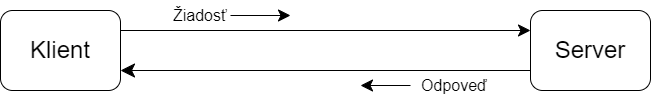
\includegraphics[scale=0.6]{obrazky-figures/http-client-server.png}
    \caption{\centering Vizualizácia konceptu komunikácie pomocou protokolu HTTP. Klient zasiela požiadavku na server a server mu naspäť posiela odpoveď.}
    \label{fig:http-client-server}
\end{center}
\end{figure}

Správy HTTP protokolu sú štruktúrované bloky textu. 
ABNF...
Správa nadväzujúca HTTP spojenie --- žiadosť, má nasledovný obsah:
\begin{enumerate}
    \item metódu
    \item cestu k požadovanému dokumentu
    \item verziu protokolu HTTP použitého na nadviazanie komunikácie
    \item \textbf{HTTP hlavičky}
    \item prípadný obsah žiadosti
\end{enumerate}


\begin{figure}[htb]
\begin{center}
    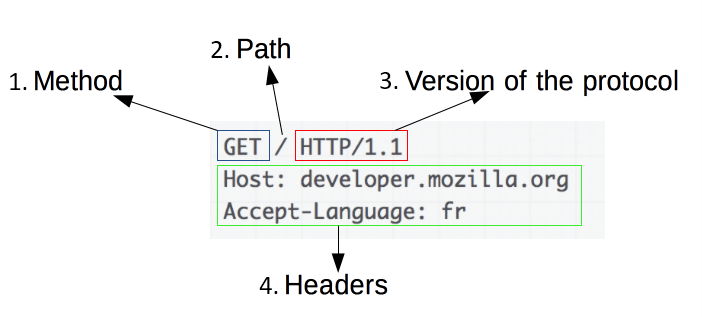
\includegraphics[scale=0.6]{obrazky-figures/http_request.png}
    \caption{\centering Vizualizácia konceptu komunikácie pomocou protokolu HTTP. Klient zasiela požiadavku na server a server mu naspäť posiela odpoveď.}
    \label{fig:http-request}
\end{center}
\end{figure}

% \# Komunikácia
% Hlavičky
% Pod-zdroje
% Status

% Endpoint...
% HTTPS

% \# Existujúce komunikačné riešenia
% Webová stránka
%     Webová podstránka
%     Priamy Odkaz                    OK
%     Spätný Odkaz ???
% Dosiahnuteľnosť Web Serveru

% Network Partition Key ??
% https://httpwg.org/specs/rfc7230.html, https://httpwg.org/specs/rfc7231.html
% Security - HTTPS, https://www.w3.org/TR/secure-contexts/

\subsection{Domény}
% DOMENY
% DNS ?

\subsection{Hľadaný dokument a jeho obsah}
% Web Stranka
% HTML - https://dom.spec.whatwg.org/, https://html.spec.whatwg.org/multipage/
% Media Type
% JSON spec = https://www.rfc-editor.org/rfc/rfc7159

\subsection{Webový prehliadač}
% JS - https://tc39.es/ecma262/multipage/


\section{Zlyhania v komunikácií Klient-Server}
\begin{itemize}
    \item General intro and info
    \item DNS
    \item Transport
    \item Application
    \item Special
    \item Web Reliability
    \item Existujúce riešenia
\end{itemize}

\section{Report API}
\begin{itemize}
    \item Všeobecná náväznosť na zlyhania komunikácie
    \item Cieľ
    \item Ako funguje
    \item Konfigurácia
    \item Príklady
    \item Možnosti reálneho využitia (konkrétna náväznosť na NEL)
\end{itemize}

\section{Network Error Logging}
\begin{itemize}
    \item Cieľ
    \item Ako zapadá do a ako využíva predošle spomenuté koncepty
    \item Ako funguje
    \item Konfigurácia
    \item Príklady
\end{itemize}



\section{OLD CONTENT}
V tejto kapitole popisujem problematiku, v ktorej sa táto práca venuje. Jedná sa tu o možné nástrahy pri komunikácií typu klient-server,
ktoré môžu nastať a spôsobiť probmlémy ako napríklad nedosiahnuteľnosť servera, s ktorým klient komunikáciu pôvodne nadviazal.
O takýchto a podobných problémoch sa server ziaľ nemá ako dozvedieť, a preto vzniká potreba nájsť nejaký spôsob ako takéto problémy pri ich
vzniku identifikovať a nahlásiť formou štruktúrovanej správy vývojárom zodpovedným za prevádzku daného servera. V prípade, že 
na problém takto poukázané, v nasledujúcich krokoch je možné postaviť sa k nemu s vhodnými protiopatreniami a úspešne ho odstrániť, a teda 
tak zároveň aj znovuspojazdniť predtým nefunkčnú komunkikáciu s klientami, u ktorých sa tento problém prejavoval.
\\
V tejto kapitole začnem s úvodom do širšieh spektra zavedenej problematiky, kde spomeniem technológie s podobným účelom 
ako Network Error Logging (ďalej označovaný iba ako NEL), aké nedostatky aktuálneho stavu problematiky riešia, no hlavne, aké majú nedostatky. 
Tým sa prepracujem k podstate a motivácií k nasadeniu samotného NEL-u a ďalších technológií priamo súvisiacich s ním. 
Jedná sa tu čisto o teoretický základ nutný pre pochopenie nasledujúcich sekcií tejto práce. 
Aktuálny stav využívania technológií spomínaných nižšie bude uvedený a detailne rozpísaný v kapitole \ref{related-work}.

\section{Všeobecná problematika zlyhaní v komunikáciach typu klient-server}

Aké problémy môžu nastať
\\
Ako sa to prejavuje
\\
Dôkaz, že server takéto problémy nedokáže detekovať

\section{Monitoriovanie spoľahlivosti webových služieb}

Sekcia bude vyplývať z článku priloženého k odporučenej literatúre zadania tejto BP \cite{nel-client-side-measurement-e2e-reliability}
\\
Existujúce populárne spôsoby riešenia uvedených problémov - napr: DVP, JavaScript...
\\
Aké problémy tieto riešenia stále nepokrývajú - napr. JavaScript sa vôbec nemusí spustiť (klient ho neobdrží od servera).
\\
Motivácia používania NEL - aké aktuálne riešenia ponúka pre možné chyby a perspektíva do budúcnosti.

\todo{Table 1: Properties satisfied by different approaches for detecting service reachability problems at scale.}

Odkaz na Table 1 - Jednou z motivácií pre vývoj štandardu NEL bolo, že ako jediný by bol schopný presne vyčísliť koľko klientov je
v danom čase (aktuálne) afektovaných výpadkom v komunikácií. Práve táto schopnosť ručí za pridanú hodnotu korektného určenia závažnosti,
tým pádom aj priority konkrétneho zlyhania. Správci serveru, ktorý interne používa NEL, majú dostatočný prehľad o stave siete a na základe 
toho môžu rozhodovať o tom, kam zamerajú svoje úsilie o riešenie závad.    

\section{Network Error Logging}

\todo{Náhľad na NEL z hladiska jeho špecifikácie}

NEL je štandard pre zachytávanie a získavanie chýb a zlyhaní na úrovni webového prehliadača navrhnutý organizáciou World Wide Web 
Consortium (ďalej v skratke iba W3C). Tento štandard bol prvýkrát popísaný v článku publikovanom 11/02/2014 a je dodnes aktualizovávaný
s tým, že posledná verzia jeho špecifikácie bola vydaná práve v dobe vzniku tejto bakalárskej práce, a to presne 5/10/2023. 

Hlavným cieľom NEL je poskytovať prevádzkovateľom webových serverov priamy pohľad na chybové stavy, ktoré môžu vzniknúť pri snahe 
klientských aplikácií komunikovať s nimi. Pri takejto klient-server komunikácií môže nastať hneď niekoľko kategórií problémov, 
kde v každej z nich si zaslúžia jednotlivé chyby svoje vysvetlenie. Dôležité je, že server v obyčajnom scenári takejto komunikácie 
nemá žiadnu možnosť dostať sa k informácií o tom, že sa niečo pokazilo, ani čo konkrétne bol samotný problém. Práve toto je cieľom 
napraviť pre tento štandard a tým pádom sa tvorcom tejto technológie jedná o postupné zvýšenie dostupnosti služieb poskytovaných 
na internete sprevádzkovaním NEL na svojich webových serveroch.

V nasledujúcich sekciách chcem vysvetliť jednotlivé detaily týkajúce sa tejto technológie, ktoré sú naprosto potrebné k porozumeniu 
implementačnej časti tejto práce - kapitole č.\ref{analysis-and-its-results}. Pokiaľ nebude uvedené inak, v tejto kapitole čerpám hlavne 
z poslednej dostupnej verzie dokumentu špecifikácie NEL\cite{W3C-NEL}.

\subsection{Základný model NEL}
\todo{Špecifikácia NEL, ktorá je jednoznačne potrebná pre účel pochopenia implementačnej časti (analýzy)} 

NEL je možné využiť pri komunikácií klienta so serverom pomocou protokolu HTTP. Jeho funkcionalita je zapracovaná do užívateľských 
prehliadačov založených na open-source?? distribúcií projektu \textbf{Chromium}, a to menovite napríklad: Google Chrome, Opera alebo 
Microsoft Edge. \todo{CITE}

Jeho vnútorné mechanizmy sú spustené práve vtedy, keď server pri vyhotovovaní novej požiadavky zašle v svojej odpovedi spolu s ostatnými 
aj hlavičku \code{NEL}. Tento proces sa nazýva \textbf{Policy delivery} a sprostredkuje dohodu o zbieraní, udržiavaní a nahlasovaní chýb 
vzniknutých pri komunikácií. Samotné politiky sú popísané vo väčšom detaile v sekcií \ref{nel-policies}.
\\
\\
Hlavička \code{NEL} vo svojej najjednoduchšej podobe musí obsahovať nasledovné položky: 

\begin{itemize}
    \item \code{report\textunderscore to} - menom označená skupina zberačov reportov (collerctors, viď \ref{reporting-api}) 
    \item \code{max\textunderscore age} - doba platnosti zaslanej politiky NEL
\end{itemize}

Tieto hlavičky musia byť zadané vo formáte \code{application\textbackslash json}, takže ukážkový obsah HTTP hlavičky NEL môže vyzerať 
napríklad takto:

\begin{lstlisting}[caption={Ukážka obsahu najjednoduchšej/minimálnej HTTP hlavičky NEL. Akékoľvek chyby budú hlásené do skupiny 
    \code{network-errors} po dobu platnosti tejto politiky, ktorá bola nastavená na 7 dní (604 800 / 60s / 60min / 24h)}]

{"report_to": "network-errors", "max_age": 604800}

\end{lstlisting}
% \label{nel-simple-example}
%\todo{center only the lstlisting without the caption}
%\\
\todo{V návrhu NEL je v detaile opísané, ako požiadavky na bezpečnosť ovplyvnili jeho návrh a funkcionalitu. Toto je nutné spomenúť, no myslím,
že sa v tejto práci tomu nie je potreba venovať}

\subsection{Konfigurácia}

Všetky položky, ktoré je možné v NEL hlavičke uviezť.

\subsection{Politiky a ich uskladňovanie na strane klienta}
\label{nel-policies}


\subsection{Rozšírenia plánované v budúcnosti}

Nová verzia NEL, ktorá bude schopná spolupracovať s Reporting API v1 (momentálne funguje iba s v0)



\section{Reporting API}
\label{reporting-api}

Doplnkové info, ktoré je skrátka nutné spomenúť \cite{W3C-reporting-api}
